% !TEX root =  ../main.tex
\section{MinSpareResources}

\subsection{Definition}

\subsubsection{Signature} \cstr{minSpareResources(s : set<server>, rc : string, n : number)}

\begin{itemize}
\item \cstr{s} : a non-empty set of servers for a meaningful constraint.
\item \cstr{rc} : a resource identifier such as \cstr{mem}, \cstr{ucpu}, \cstr{pcpu} or \cstr{nodes} to identify the physical memory,
the computational capacity, the physical CPUs or the node itself, respectively.
\item \cstr{n} : a positive number
\end{itemize}

The \cstr{minSpareResources} restricts to at least \cstr{n}, the number of free resources directly
available for VMs on the online servers in \cstr{s}. Servers in the \st{Offline} state are ignored.

\classification{minSpareResources}{datacenter administrator}{Resource allocation}{Resource management,Power saving,Capacity planning}

\subsubsection{Usage}

This constraint deserves the control of a power saving strategy. The most effective solution
to reduce the energy consumption of a non-saturated datacenter is to turn off unused servers
and to turn them on and off depending on the load variation.
When a load spike arise, it may be a necessary to put some servers online to make their resources available to the VMs.~\cite{hermenier-xhpc06,vmware-dpm}
The time to boot the awaited servers may however be significant and alter the reactivity of the datacenter
when it faces an emergency situations. One solution is to let online a controlled number
of \emph{spare} resources that can be used instantly to absorb the load increase.
A datacenter administrator may then use  \cstr{minSpareResources} constraints
to control the minimum number of free resources to let directly available while the other unused resources are still manageable by the power saving strategy.

\subsubsection{Example}

Figure~\ref{fig: minSpareResources} depicts a sample reconfiguration between a source and a destination configuration where each server provides 8 unit of CPU and 7 unit of memory resources to VMs. During the reconfiguration, several relocations have been performed and the server \cstr{N3} has been turned off to save power. In this setting, the following \cstr{minSpareResources} constraints were considered:

\begin{figure}[htb]
\centering
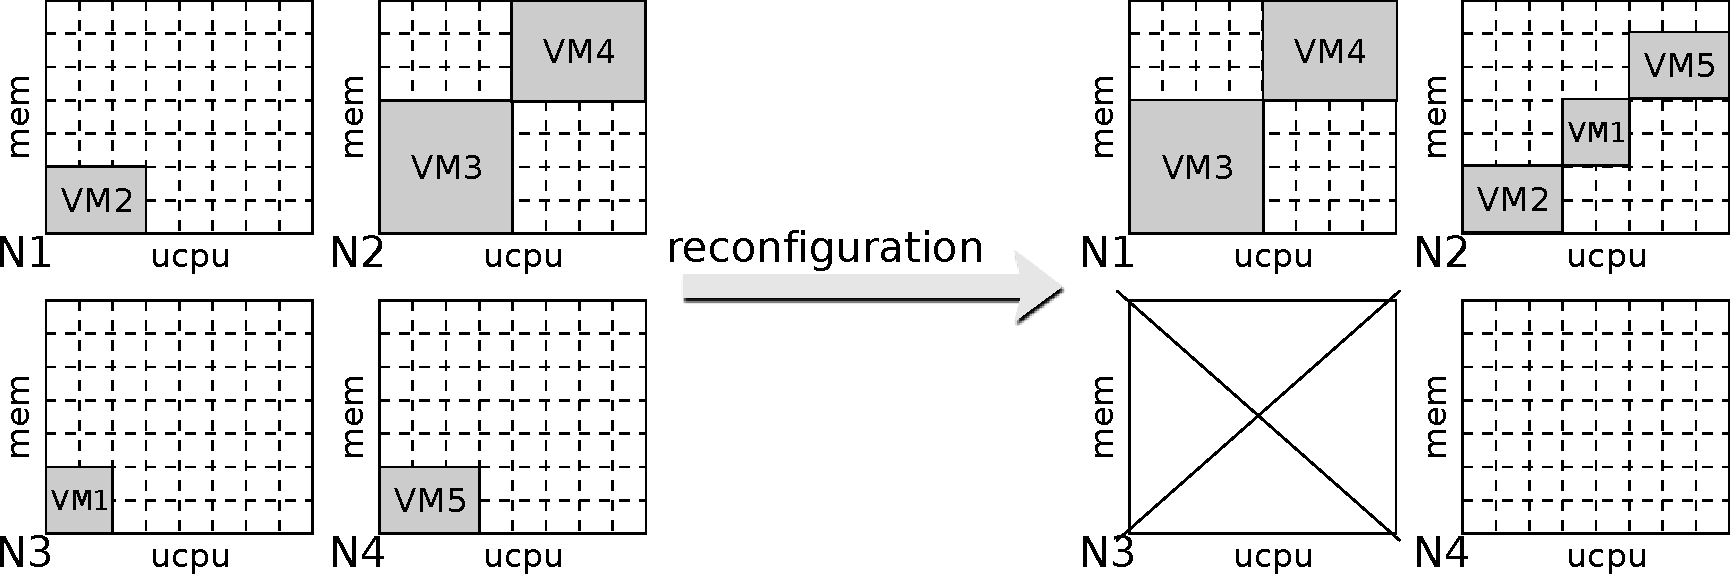
\includegraphics[width=\textwidth]{img/minSpareResources}
\caption{A reconfiguration motivated by \cstr{minSpareResources} constraints.}\label{fig: minSpareResources}
\end{figure}

\begin{itemize}

\item \cstr{minSpareResouces(\{N1,N2,N3\},"ucpu",0)}. This constraint was satisfied in the source configuration as 11 unit of CPU were directly available to the running VMs. The constraint is also satisfied in the destination configuration as 0 unit are available: resources on \cstr{N3} are not considered as it is in the \st{offline} state.

\item \cstr{minSpareResources(\{N2\},"mem",1)}. This constraint was not satisfied in the source configuration as no memory resources were available on \cstr{N2}. The reconfiguration process fixed that violation by relocating away \cstr{VM4} and \cstr{VM3} and host \cstr{VM2},\cstr{VM1}, and \cstr{VM5} while keeping one unity of memory resources directly available.

\item \cstr{minSpareResources(\{N2,N3,N4\},"node",1)}. This constraint was not satisfied in the source configuration as no servers were idle. The reconfiguration fixed this violation by relocating all the VMs on \cstr{N4} to other servers while keeping it in the \st{Online} state.

\end{itemize}

\fullVersion{
\subsection{Model}

The \cstr{noIdleOnlines} constraint is modeled in terms of the RPs variable by restricting
the state variable of each involved server to 0 depending on the number of VMs running
on the servers.

\begin{equation*}
\begin{split}
\forall N \in \mathcal{N},\ offline(N) & \triangleq\\
&	\forall n_i \in N, 
\sum_{d_i |�v_i \in \mathcal{V}} d_i = 0 \imply n_i^q = 0
\end{split}
\end{equation*}

\subsection{Violation detection}

To compute the list of violating elements, it is a necessary to check for each of 
the involved  server that are still online without running any VMs. This indicates
the violating servers.


\subsection{Availability}

\subsubsection{In {\btrp}}

The constraint is available in {\btrp} under the name \cstr{noIdleOnlines}.
To check whether a server is running a VM or not, we rely on the variable
indicating its memory usage. When this variable equals 0, then it is considered
the server does not host any VM and has to be turned off.

\begin{equation*}
\begin{split}
\forall N \in \mathcal{N},\ offline(N) & \triangleq\\
&	\forall n_i \in N,  eq(n_i^{mem}, 0) \imply eq(n_i^q, 0)
\end{split}
\end{equation*}
}

\subsection{See also}

\subsubsection{Related Constraints}
\begin{itemize}
\item \cstrref{maxSpareResources}: This constraint controls the maximum number of unused but available resources.
\end{itemize}


\printListOfInheritance{minSpareResources}
%
%\begin{itemize}
%\item \hyperref[cstr: offline]{\cstr{offline}}: The turn off servers in any condition.
%\end{itemize}